%%%%%%%%%%%%%%%%%%%%%%%%%%%%%%%%%%%%%%%%%
% University/School Laboratory Report
% LaTeX Template
% Version 3.1 (25/3/14)
%
% This template has been downloaded from:
% http://www.LaTeXTemplates.com
%
% Original author:
% Linux and Unix Users Group at Virginia Tech Wiki 
% (https://vtluug.org/wiki/Example_LaTeX_chem_lab_report)
%
% License:
% CC BY-NC-SA 3.0 (http://creativecommons.org/licenses/by-nc-sa/3.0/)
%
%%%%%%%%%%%%%%%%%%%%%%%%%%%%%%%%%%%%%%%%%

%----------------------------------------------------------------------------------------
%	PACKAGES AND DOCUMENT CONFIGURATIONS
%----------------------------------------------------------------------------------------

\documentclass{report}

\usepackage[version=3]{mhchem} % Package for chemical equation typesetting
\usepackage{siunitx} % Provides the \SI{}{} and \si{} command for typesetting SI units
\usepackage{graphicx} % Required for the inclusion of images
\usepackage{hyperref}

\usepackage{amsmath} % Required for some math elements 
\usepackage{indentfirst}
\usepackage{dirtytalk}
\usepackage{titlesec}

\title{Enhancing deck building AI with Genetic Algorithms and Neural Networks} % Title
\titleformat{\chapter}{\normalfont\LARGE\bfseries}{\thechapter.}{18pt}{\LARGE\bfseries}
\titleformat*{\subsection}{\large}
\titleformat*{\subsubsection}{\normalfont}
\author{Callum \textsc{Roberts}} % Author name
\setcounter{secnumdepth}{4}


\renewcommand{\labelenumi}{\alph{enumi}.} % Make numbering in the enumerate environment by letter rather than number (e.g. section 6)
\bibliographystyle{IEEEtran}
%\usepackage{times} % Uncomment to use the Times New Roman font

%----------------------------------------------------------------------------------------
%	DOCUMENT INFORMATION
%----------------------------------------------------------------------------------------



\author{Callum \textsc{Roberts}} % Author name

\date{\today} % Date for the report

\begin{document}

\maketitle % Insert the title, author and date

% If you wish to include an abstract, uncomment the lines below
% \begin{abstract}
% Abstract text
% \end{abstract}

%----------------------------------------------------------------------------------------
%	SECTION 1
%----------------------------------------------------------------------------------------

\chapter{Literature Review}
The purpose of this literature review is define the technologies used in the field of artificial intelligence for building a deck in Hearthstone. To introduce, and compare previous works to determine their strengths and weaknesses. A review of the literature is valuable in understanding important aspects of a research area \cite{}. The structure of this literature review is as follows: An initial section will detail the background of the project, explaining the fundamentals of Hearthstone and deck building. Following that will be the introduction to the project,  motivation and research questions. Finally we will have the core technologies used for similar projects.
\section{Background}
	For the benefit of the reader, this section will introduce the basics of Hearthstone. It will emphasise the deck building aspect of the game including practices used by players.  
\subsection{Collectible Card Games}
	Collectible Card Games (CCG)\footnote{\url{https://en.wikipedia.org/wiki/Collectible_card_game}} are a sub-genre of card games introduced in 1993 by Magic: The Gathering \footnote{\url{https://en.wikipedia.org/wiki/Magic:_The_Gathering}}. It requires a player to make a custom deck to play, it mixes trading cards with strategy and deck building features. CCGs are usually defined as a turn based game, where each player acquires their own collection of cards through the purchasing of "starter decks" for beginners or "booster packs" containing a small amount of random cards from a {\it{pool}} of cards usually referred to as an expansion. The aim is to build an efficient deck that can account for the randomness that come from the nature of card games, to predict and play around your opponents actions to ultimately beat them. Some CCGs can prove to be lucrative for players as cards have a value intrinsic to their rarity and demand \footnote{\url{https://www.cardmarket.com/en/Magic/}}, this makes building the perfect deck rather difficult and usually costly.
\subsection{Hearthstone}
	Hearthstone: Heroes of Warcraft is a CCG developed by Blizzard entertainment in 2013 \cite{HS}, but with the twist of it being entirely digital, there is no physical version of the game. This choice unlocks potential for gameplay features that could not be implemented, in exchange for the tradability of the cards. \\ \\ \\
\begin{figure}[h]
\centering
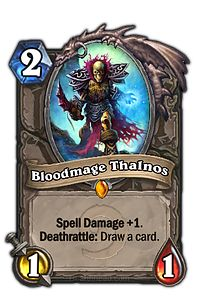
\includegraphics[width=0.25\textwidth]{thalnos}
\caption{Example of a Legendary Hearthstone card - Source \href{https://www.pinterest.fr/pin/573716440004576557/}{here}
\label{card}
}
\end{figure}

	\indent Two players face off wielding each a deck of their own making. Decks consist of no more, no less than 30 cards. Players then take it in turns to play their cards, the objective being to reduce the other players health to 0. On each of the players turns that player draws a card and gains a “Mana Crystal” up to a maximum of 10 (crystals are refreshed every turn), these crystals are expended to cast a card from the player's hand. Before a match each player chooses to embody a class (such as Mage, Warrior, Rogue, Druid, etc…), each class has specific cards only they can add into their deck, these are adequately named “Class Cards”, these are accompanied by “Neutral Cards” that any class can use. Classes also have access to an ability unique to them called a {\it{hero power}}. \\
	
\begin{figure}[h]
\centering
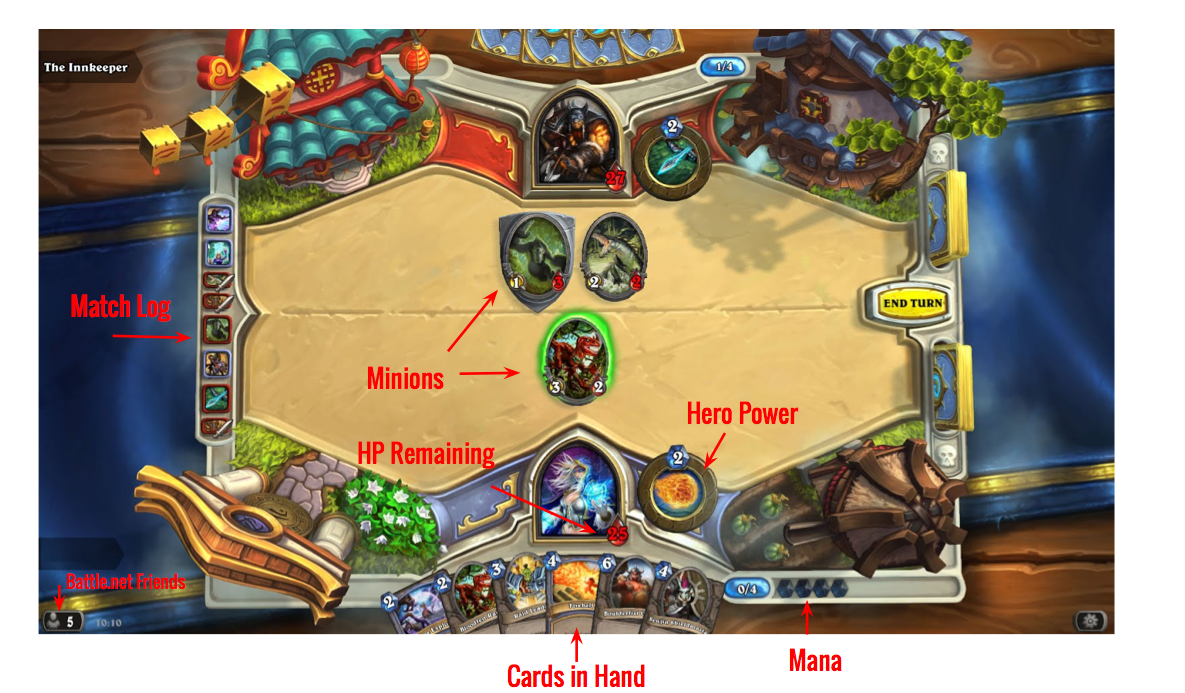
\includegraphics[width=1\textwidth]{hearthstonegameboard}
\caption{Example of a Hearthstone board - Source
 \href{https://bothgunsblazingblog.wordpress.com/2014/06/22/hearthstone-analysis-and-deconstruction/}{here}  }
 \label{board}
\end{figure}
	
	Each card in the game has a “mana” cost which shows how many mana crystals are needed to cast that card. They also have a card type, rarity and an effect. In a deck, players can put duplicates of the same card (up to 2) except for "Legendary Cards" (figure \ref{card}) that are limited to 1 because of their powerful effects.  Players have a “Collection”, where the cards they own are stored, to get new cards players can buy card packs with gold, the in-game currency of Hearthstone. Gold is earned slowly through quests, winning and events, it can however be sped up through the purchase of gold with real life currency. Players can also choose to "Disenchant" their duplicate cards to gain another in-game currency called "Dust" which can be used to create a card of the players choosing\footnote{\url{https://hearthstone.gamepedia.com/Crafting}}.


\subsection{Deck Building}
	In the world of CCGs there is a long standing debate on how to measure the skill of a player, although card games involves luck and circumstance, it is believed that there is a degree of strategy in the building of decks and in the execution of decks whether it is just a slight increase in win probability or a fundamental to winning \cite{SvsL}. However the debate stems from which is the most important, the building aspect or the execution aspect of CCGs
	\cite{BvsP}
	\subsubsection{Metagame}
	Hearthstone is a game with lots of complex systems that are influenced by many factors, mainly due to the large amount of cards and different playable heroes. In a game where there are lots of variables, players try to rank cards, heroes and combination as to increase their chances to win. This phenomenon creates decks from a "pool" of top rated cards, leaving out the mediocre, forcing players to use these top rated decks in order to have a better chance of winning, or be put at a disadvantage. The result is what is called the "Metagame" or {\it{meta}} for short. Blizzard release updates to the game frequently through "expansions" which add a variety of new cards to keep the game fresh. Shifts in the meta occur when these expansions are added, players experiment to find better combinations over time. However better cards may not be added, and changes in the meta may not occur, this dissuades players from continuing or returning to play knowing that they have already experienced all that they can. To avoid that Hearthstone has implemented two game modes, one which has the cards added from the past two years are the only available, and another mode that allows all cards. Whilst this method helped, it still doesn't put a stop to the possibility of a stale meta. Researchers have done studies on how to evolve the meta through AI means, by {\it{balancing}} powerful cards ({Fernando et al}) \cite{EvolveMeta}. Balancing a card means to adjust the power of said card as to make it more or less viable in the current game environment. Fernando et al. discussed the idea that around 50\% of Hearthstone's meta is derived from match-ups which is the win probability two deck have against each other, a favourable match-up being the one with the highest win probability or known in the community as {\it{win rate}}.  
\subsubsection{Mana Curve}
	Theorycrafting is a term used widely in many video games, it designates a mathematical analysis of a games core mechanics to attempt to discover new strategies or combinations that could rival the current ones. Hearthstone is one such game, a large portion of the player base enjoys theorycrafting new decks that may {\it{break}} the meta, as in cause a fundamental shift of the current metagame. These players rely on fundamentals or schematics that are used as a guideline in building a new deck. The {\it{mana curve}} \footnote{\url{http://hearthstone.gamepedia.com/Mana_curve}} is one such fundamental, it exists in all decks built in the game. Every card in Hearthstone has a cost, this cost determines the power of the card, a low cost card will be weaker than a higher cost card since it would cost less resources to cast. This {\it{mana curve}} is a histogram of each card plotted by cost, it allows players to visualize how expensive in resources their deck is and to determine the deck's archetype. 
\begin{figure}[h]
\centering
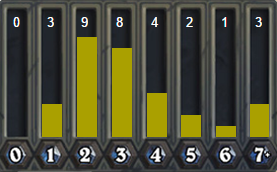
\includegraphics[width=0.5\textwidth]{mana_curve}
\caption{Example of a Mana Curve  - Source
 \href{https://hearthstone.judgehype.com/deck-mage-tempo-ladder-legendaire-tgt-gvg/}{here}  }
\label{board}
\end{figure}
\subsubsection{Archetype}
\label{archetypes}
	The word archetype is derived from the Greek word {\it{archétypon}} which means "beginning, origin", applied in the psychology field to categorize complex human behaviour called Jungian Archetypes \cite{Robertson2016}. This term was transposed into the deck building field of CCGs, a deck archetype is meant to categorize and describe the behaviour of the deck from a high level perspective, forgoing the need to play the deck to learn the strategy of the deck. In Hearthstone, most decks can be categorized by three main archetypes \cite{Judlick}:
\begin{itemize}

\item Aggro decks are the aggressive decks meant to defeat an opponent as quickly as possible, as consequence the mana curve of such decks is focused towards the cheaper side of the histogram. Their power comes in the early turns, but they quickly become weaker to the other archetypes as the turns go on.
\item Control decks are decks meant to control the state of the board the use of expensive cards, they tend to generate a lot of cards and have a wide range of card choices. The mana curve of such an archetype is towards the expensive end of the curve. They tend to have a few cards to play early in the game, but have a multitude of win conditions later on in the turns.

\item Mid-range decks are situated in the middle of the two other archetypes, focusing mainly on the mid game, their win conditions are stronger than the aggro decks but weaker than the control decks. Their mana curve peaks in the middle of the histogram.
\end{itemize}

Hearthstone also has other archetypes that cover a shorter scale, they are usually introduced in the newer expansions and rotate out of the normal game after a couple of years \cite{Standard}. For example a highlander archetype is a deck with 30 unique cards. Archetypes are formed around specific cards with win conditions\footnote{\url{https://playhearthstone.com/en-us/news/21363038}}, meaning that they have the power to win the game. So in the example given in a highlander deck there would be a card that has an effect that triggers from having only unique copies in the deck.
 
\subsubsection{Resource Cost}
	In CCGs cards have a certain cost to use, in Hearthstone that cost is mana which regenerates every turn. The cost of a card is determined by the power of said card, if it has a powerful effect, has decent attack and defence values or even both. This cost will determine how late into the game a card can be played. However a card that costs a lot can be considered weak and a low cost card can be considered strong. The power of a card is determined through the resource cost, an invisible value that is hard to calculate and a subject of study \cite{Zuin2019}. Although the Zuin et al. study was used to predict the cost of a card in Magic: The Gathering, the resource calculation is still present, it poses a good solution to the balancing of the metagame and would be adaptable to Hearthstone. A card is considered efficient if the theoretical resource cost is higher than the current mana cost, and would be inefficient if the resource cost were to be lower than the mana cost. The resource cost of a card is something that may need to be considered when developing an AI for building decks. Stiegler et al. \cite{Stiegler2017} applied a similar theory to design a deck building AI based on a utility system that classified cards based on resource cost effectiveness, mana curve and synergies.
\section{Project Introduction}
	 The rising popularity of Hearthstone has attracted a lot of new players reaching over 100 million accounts in 2018 \cite{100mil}, however due to the nature of collecting cards in the game some will not have the required cards to build the most popular decks. The game is free, anyone can download it, however a lot of the content is locked behind a paywall\footnote{\url{https://en.wikipedia.org/wiki/Paywall}}. Whilst it is possible to earn cards by earning "gold", the games currency, through winning games and completing quests \footnote{\url{https://hearthstone.gamepedia.com/Gold}}, it becomes a time consuming ordeal that requires a lot of spare time to invest. With new expansions being added regularly, the game seems to become a never ending grind, unless you decide to pay real money to acquire "gold". This is where the term "pay-to-win" is used to describe Hearthstone \cite{Howard2019}, meaning that to get the most enjoyment and the highest chance to win, the player must spend money or be disadvantaged. The goal of this honours project is to create an AI that builds decks from a  collection of cards, incomplete or otherwise in order to close improve the game experience for players that are not willing to pay. For players that do own a large collection of cards it can also provide fresh new decks to play that differ from the popular ones.
\subsection{Related Works}
	Video games are the ideal tool for the training of Artificial Intelligence. The virtual space that a game provides is a realistic environment with a limited amount of information available \cite{Sweetser2002} allowing control and knowledge over the behaviour of the AI. Hearthstone is a game that provides a platform for a wide variety of AI that differ from the AI-benchmark games such as Chess or Go. Hoover et al. \cite{Hoover2019} classifies Hearthstone AI into specialized categories: 
\begin{itemize}
\item Game Playing AI, self explanatory, this form of AI is designed to play the game. Generally tree search algorithms are used, Monte Carlo Tree Search (MTCS) in particular. However this method is rather ineffective in a Hearthstone due to the amount of hidden information and limited visibility of the AI . Developers of Hearthstone simulators, such as {\it{MetaStone}}\footnote{\url{http://www.demilich.net/}} tend to use a greedy approach to compensate \cite{yannakakis2018artificial}. Some researchers attempt to use variations of MCTS and heuristics to work around the limited information \cite{Janusz2017}\cite{Miguel2017}\cite{Swiechowski2018}.
\item Developer Assiting AI, this AI help with certain issues that developers could have. Since Hearthstone has hundreds of cards, it is challenging to design cards with new flavour that are not identical to previously printed cards. Could there be a way to generate inspiration? Woolf "minimaxir" Max\footnote{\url{https://minimaxir.com/apps/gpt2-mtg/}} created an API that generates Magic: The Gathering cards\footnote{For example cards: \url{https://github.com/minimaxir/mtg-gpt-2-cloud-run/tree/master/generated_card_dumps}} using a transformer language model\footnote{\url{https://openai.com/blog/tags/gpt-2/}} for such a purpose. Another possible use is for balancing the game, since maintaining game balance when creating additional cards may created unfair combinations, or render some cards useless\cite{EvolveMeta}.
\item Deck Building AI, they create decks for the player or another AI to use, most commonly created with Evolutionary Algorithms\cite{Back1996}. It has the inherent advantage of being usable in conjunction with other AI, such combinations help ascertain potential balance issues without human bias involved. Since this is the main topic of this paper, further in-depth explanation will be provided in the body. 
\end{itemize}

	Whilst all these AI are used in the context of Hearthstone, they are utilized for different aspects of the game therefore proving that Hearthstone is a platform with a constant influx of AI challenges to be met, a prime example is with the additional {\it{battlegrounds}} gamemode\footnote{\url{https://hearthstone.gamepedia.com/Battlegrounds}}, a variation of the game where the creatures attack on their own automatically, then completing your board as you progress between rounds. This alteration of the way the game is played and surely will be subject of a paper in the future. 

\subsection{Research Questions}
Research Questions are essential to any methodical research, it is the first step in any project and fundamental to any successful project. Kowalczyk\cite{Kowalczyk2013} described Research Questions as a metaphor for a house: \say{Your data collection forms the walls, and your hypothesis that guides your data collection is the foundation. So, what is the research question? It is the ground beneath the foundation. It is what everything in a research project is built on. Without a question, you can't have a hypothesis. Without the hypothesis, you won't know how to study what you're interested in.}
The research questions in this literature review are defined as:

\begin{itemize}
\item \textbf{RQ1:} What are the current best deck-building techniques in Hearthstone?
\item \textbf{RQ2:} What are the strengths and weaknesses of the different techniques?
\item \textbf{RQ3:} With our findings, what techniques can be applied to optimize the deck-building problem in Hearthstone?
\end{itemize}

\subsection{Assistance Systems}
Despite AI being widely used in Hearthstone for research purposes, it is against Blizzard's Terms of Service (ToS) to use game playing AI in Hearthstone (Section 1.C.II)\footnote{\url{https://www.blizzard.com/en-us/legal/fba4d00f-c7e4-4883-b8b9-1b4500a402ea/blizzard-end-user-license-agreement}}. However, a surge of Hearthstone deck tracking software \footnote{Some software examples: \url{https://hsreplay.net/downloads/?hl=en} \\ \url{https://go.overwolf.com/firestone-app/} \\ \url{http://hearthstonetracker.com/}  \\ \url{https://trackobot.com/}} are being used by players without being banned. So how do players use this kind of software without violating ToS? It was revealed that turning on debug logs would provide enough information for these systems without breaking ToS \cite{Flipperbw2014}. Which birthed a whole sub-genre of AI coined as "Assistance Systems" designed to be used to assist the player without it being considered cheating. This brought on the creation of deck trackers, which mentioned above track which cards each player has used and tracks statistics. Whilst deck trackers are not AI since they just real logs, Bursztein \cite{Bursztein2016} used this system to create an AI that predicted what cards the opponent would play in future turns, and used this predictor AI to climb to \textit{legend} rank (the highest rank in competitive mode\footnote{\url{https://hearthstone.gamepedia.com/Ranked}}). Whilst it was not against ToS to use it, when they presented the tool, Blizzard reached out to them and asked them not to release the code as it was \textit{game breaking}. The effectiveness of the tool was however limited to later turns, the accuracy is much lower (going as low as 50\%) in first turns and becomes more accurate each turn. Some of the most crucial turns for some archetypes are in those early turns, so this AI would only maximise effectiveness for the \textit{Control} Archetype (\ref{archetypes}). \\
\indent Other assistance algorithms include Hearthstones Area game mode\footnote{\url{https://hearthstone.gamepedia.com/Arena}}, a mode where the player drafts a deck one card at a time by selecting 1 of 3 possible choices from a pool of cards, using Apriori algorithms \cite{Agrawal1994} such as HearthArena\footnote{\url{https://www.heartharena.com/}} to make suggestions based on  data from a diverse range of high quality decks created by player and/or deck building algorithms\cite{MapElites}. However this sort of algorithm would be only be useful in an environment where the player cannot select their cards. \\ 

The use of assistance systems is interesting but still requires the interactivity of a human party to function. The advantage to assistance systems is the ethical and legal implementation from it. The disadvantages such as the low accuracy rate of the prediction tool in earlier stages of the game, or the limited usability of the Apriori algorithm makes it difficult to be used in a standard deck building format.

\section{Genetic Algorithm}
Developed AI algorithms often draw inspiration from biology\cite{Eiben2015}, Genetic Algorithms (GA) is an example of this. GAs are a subset of Evolutionary Algorithms (EA) that base their training process the same way nature does, biological evolution through natural selection (Figure \ref{ea}).  A population of solutions each with a set of properties (chromosomes in nature) which are mutable is randomly generated. Each iteration or \textit{generation} the algorithm selects the most fit individuals of the population using a fitness function, then the most fit are used to form the next generation, some mutations of properties may occur in some of the population. The algorithm ends when either the correct fitness level is achieved  or when the number of set generations is reached\cite{Whitley1994}. GAs are stochastic in nature, meaning that a single iteration would not be sufficient to provide significant statistical results \cite{Merelo2015}. The process is reminiscent of Charles Darwin's theory of evolution\footnote{\url{https://en.wikipedia.org/wiki/Natural_selection}} and proves to be effective in optimization problems\cite{Eiben2015}.  \begin{figure}[h]
\centering
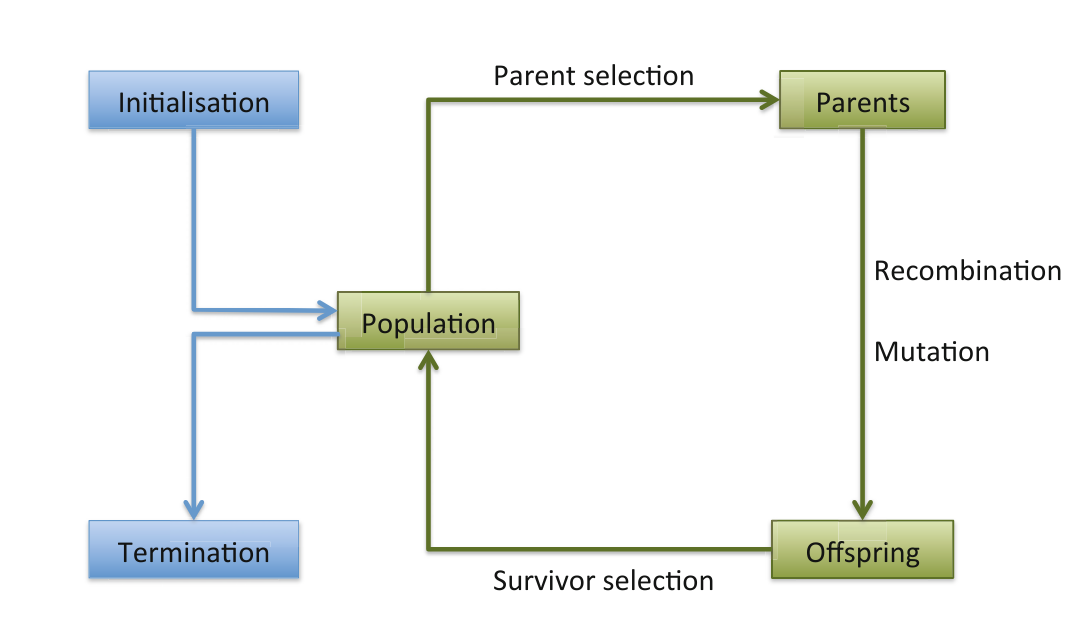
\includegraphics[width=1\textwidth]{EAFlowchart}
\caption{Evolutionary Algorithm Flowchart \cite{Eiben2015}  }
\label{ea}
\end{figure}
This algorithm is the most frequently used for deck building problems \cite{Fludal2017}\cite{GarciaSanchez2016}\cite{GarciaSanchez2018}, although they are optimized in different ways. In GAs there exists a fitness function that determines the fitness score of an individual that is used to create the next generation, and there is the mutation function which will randomly mutate some individuals, it may or may not improve the fitness of said individual. \\ 
\indent Bjørke and Fludal \cite{Fludal2017} used a genetic algorithm to construct decks for Magic: The Gathering based of a certain pool of cards. Instead of using a fitness function that would calculate the score of a deck, they pitted each deck in that generation against each other in a tournament format using a Magic: The Gathering game simulator, each deck had the same number of games to play and they would select the most fit decks based of their winrate in the tournament. While theoretically the idea is sound, the time that it took was substantial for an unremarkable winrate (less than 60\%). With 50 matches per deck over 350 generations, it took 43 hours to execute. Due to the time it take it would be unusable for players as it would simply take too long.\\
\indent Garcia-Sanchez et al. had a similar approach using lexicographical fitness with a Hearthstone game simulator called \textit{MetaStone}\footnote{\url{https://github.com/demilich1/metastone}}, separating the fitness evaluation into three parts: One part that counted the number of victories of in 16 games, another part which determined the deck correctness (no more than 2 duplicates, only 1 legendary, etc...), last part was applying standard deviation to the number of victories, it being optimal if the deck won against every opponent \cite{GarciaSanchez2016}. The results were much better and achieved faster than Bjørke and Fludal's work\cite{Fludal2017}, however the results were not as high as they could have been, mainly due to the fitness function using \textit{MetaStone's} greedy AI to play. The decisions made by the AI would be greedy and different to that of a human player. The mutation function could also have been touched on, allowing the mutation to make smarter decisions about which cards to mutate. \\
\indent Garcia-Sanchez et al. tackled the problem once again and touched on the mutation function \cite{GarciaSanchez2018}, they developed a \textit{smart mutation} function that would replace a card in a deck with another of a similar cost (roughly ± 1). The results with the smart mutation were overall better than without it. This may solve one of the weakness of their previous work\cite{GarciaSanchez2016} but still uses the same simulator heuristic.
\section{Neural Networks}

\section{Hybrids}


%----------------------------------------------------------------------------------------
%	SECTION 3
%----------------------------------------------------------------------------------------
\section{Conclusion \& Final Thoughts}
%----------------------------------------------------------------------------------------
%	BIBLIOGRAPHY
%---------------------
\bibliography{export}


%----------------------------------------------------------------------------------------


\end{document}